\documentclass[conference]{IEEEtran}
\IEEEoverridecommandlockouts
\usepackage{cite}
\usepackage{amsmath,amssymb}
\usepackage{graphicx}
\usepackage{booktabs}
\usepackage{pgfplots}
\pgfplotsset{compat=1.16}
\usepackage[hidelinks]{hyperref}
\usepackage{xcolor}

% --- single-source the ns-3 worked-example numbers (8B tp1/pp2, ns-3/HPCC) ---
\newcommand{\stepfloor}{435.67}      % compute floor, ms (8B, DP=16)
\newcommand{\dpstep}{1--3}           % DP all-reduce step-time benefit (%) -- hidden
\newcommand{\dpflow}{2.4--3.0}       % DP all-reduce per-flow congestion (both fabrics)
\newcommand{\ppmult}{5.6}            % PP cross-stage send congestion, 8:1 Clos, DP=8
\newcommand{\ppworst}{8.7}           % worst PP flow, 8:1 Clos, DP=8
\newcommand{\fatmult}{4.1}           % PP cross-stage send congestion, 4:1 fat, DP=8
\newcommand{\ppdpfour}{3.9}          % PP cong, 8:1 Clos, DP=4
\newcommand{\ppdpsixteen}{15.2}      % PP cong, 8:1 Clos, DP=16
\newcommand{\closoverhead}{3.8}      % PS step overhead vs OCS floor, 8:1 thin Clos (stage 0)
\newcommand{\TODO}[1]{\textcolor{red}{[#1]}}

\begin{document}

\title{Workload--Network Co-Design for LLM Training:\\ A Multi-Fidelity Methodology for Precision Time and\\ Hybrid Packet/Circuit Fabrics}

\author{\IEEEauthorblockN{Sahas Munamala}
\IEEEauthorblockA{\textit{[Affiliation]}\\
munamalasahas@gmail.com}
\and
\IEEEauthorblockN{Ahmad \TODO{Surname}}
\IEEEauthorblockA{\textit{[Affiliation]}\\
\TODO{email}}}

\maketitle

\begin{abstract}
Large-scale distributed AI training increasingly stresses datacenter interconnects through repeated collective communication, including all-reduce, reduce-scatter, all-gather, and all-to-all operations. In many training regimes, a substantial fraction of step time is spent in network activity, but only the exposed portion of communication that lies on the critical path directly affects job completion time. We investigated whether precision time synchronization across training nodes, optionally combined with partial replacement of packet switches by electrical or circuit switches, can improve training performance for a given workload. Precision time may enable deterministic collective launch windows, endpoint pacing, and scheduled circuit reconfiguration, while circuit switching may benefit workloads whose communication is large, predictable, repeated, and insufficiently hidden by computation.  We analyze this question at multiple fidelities, combining analytical bounds, execution-trace replay, and packet-level network simulation. With Llama-3 8B, we find a sharp split by traffic class: data-parallel all-reduce traffic hides behind computation and is essentially unaffected (1-3\% even under heavy congestion), while pipeline inter-stage traffic on the critical path congests by up to 15.2$\times$ and grows with over-subscription and data-parallel degree. Hybrid packet switching and circuit switching fabrics pay only for specific traffic classes and operating points, which the talk maps quantitatively. The required precision-time tolerances remain within commodity optics. The resulting framework provides an actionable way to determine when precision-time scheduling and hybrid packet/circuit fabrics can reduce mean and tail training step time, and when optimized packet switching alone is likely sufficient.
\end{abstract}

\section{Introduction}
Training a large language model alternates compute with collective communication
(all-reduce, reduce-scatter, all-gather, all-to-all). It is tempting to assume faster or more
deterministic fabrics directly speed training; circuit switching and precision time
synchronization are often proposed on that basis. But job completion time responds only to the
\emph{exposed} communication on the critical path---and whether a flow is exposed is decided by
its traffic class and the operating point, \emph{before} the network is even considered. A
circuit fabric can only recover congestion on traffic that is both exposed and contended.

This paper measures, for Llama-3 8B, \emph{which} traffic a hybrid packet/circuit fabric can
help and under what conditions, separating two classes with opposite behavior. Our findings:
(i) data-parallel all-reduce overlaps with backward compute, so even \dpflow$\times$ per-flow
congestion on an over-subscribed packet fabric costs only \dpstep\% of step time---circuits are
wasted on it; (ii) pipeline cross-stage sends are on the critical path and cannot hide, and
their congestion scales steeply with the two axes that also degrade packet fabrics:
over-subscription (\fatmult$\times$ at 4:1 $\to$ \ppmult$\times$ at 8:1) and data-parallel
degree (\ppdpfour$\times$ at DP=4 $\to$ \ppdpsixteen$\times$ at DP=16); (iii) the circuit
benefit is consequently not a constant but a product of exposed-traffic class, over-subscription,
and parallelism---low single digits today, rising as allocations enter comm-bound regimes; and
(iv) the precision-time requirements are all within commodity hardware, so synchronization is not
the limiting factor---capacity is. The methodological contribution is \emph{fidelity selection}:
hidden data-parallel traffic is captured analytically, while exposed pipeline congestion must be
escalated to packet level.

\section{Method}
We synthesize each workload as a Chakra execution trace with a symbolic tensor-graph generator
validated to 0.23\% communication-volume error against a real 128-GPU H100 run; network and
system are separate configuration, so one trace drives every fabric model. We compute exposed
communication, circuit capacity, and precision requirements analytically---validated by an
artifact-free coupled DAG scheduler that reproduces the trace-driven simulator to 0.3\% and
collapses to the compute-plus-latency floor at infinite bandwidth---and measure
multilevel-fabric congestion at packet level in ns-3 with HPCC. The circuit (OCS) baseline is
a contention-free fabric; the packet (PS) baseline is an over-subscribed Clos. Both are
reported as overhead above a common compute-plus-latency floor, so the circuit-vs-packet delta
is attributable to the fabric alone. The circuit \emph{advantage} is necessarily a
packet-level quantity: a contention-free analytical baseline cannot exhibit the congestion that
circuits remove.

\section{Results}
\subsection{Communication is mostly hidden}
For Llama-3 8B at 400~Gbps, comm--compute overlap is 96.9\%; the step is 436.9~ms against a
435.67~ms compute floor, exposing only 1.2~ms. Circuit switching has at most this 1.2~ms to
recover---the result that frames everything below.

\subsection{The exposed-comm envelope}
Holding compute fixed and sweeping inter-node bandwidth (Fig.~\ref{fig:envelope}), exposed
communication stays under 1.2\% of the step above 100~Gbps---the network is hidden and packet
switching suffices---then grows super-linearly below 50~Gbps (7.3\% at 50~Gbps, 79\% at
25~Gbps). The knee at 50--100~Gbps sets a ceiling on what \emph{any} network optimization can
recover at a given operating point. The 400~Gbps point reproduces the measured InfiniBand
baseline (0.28\%, 1.2~ms), anchoring the curve.

\begin{figure}[t]
\centering
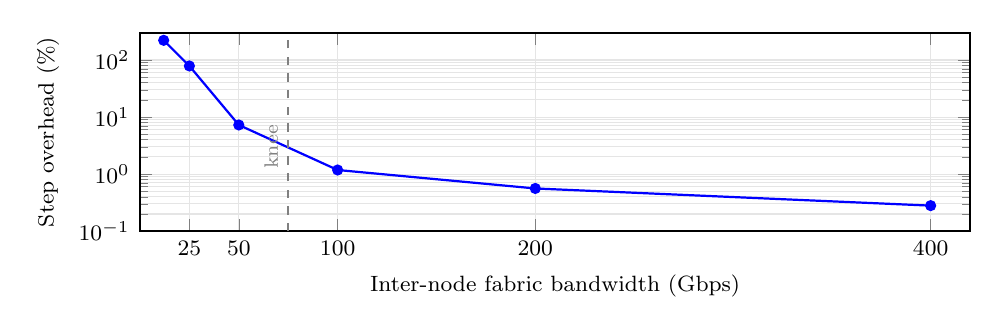
\begin{tikzpicture}
\begin{semilogyaxis}[
  width=\columnwidth, height=4.1cm,
  xlabel={Inter-node fabric bandwidth (Gbps)},
  ylabel={Step overhead (\%)},
  xmin=0, xmax=420, ymin=0.1, ymax=300,
  xtick={25,50,100,200,400},
  grid=both, grid style={gray!20},
  mark size=1.6pt, thick,
  label style={font=\footnotesize}, tick label style={font=\footnotesize},
]
\addplot[blue,mark=*] coordinates {
  (400,0.28) (200,0.56) (100,1.18) (50,7.27) (25,78.74) (12,221.69)
};
\draw[dashed,gray] (axis cs:75,0.1) -- (axis cs:75,300);
\node[font=\scriptsize,gray,rotate=90,anchor=south] at (axis cs:75,3) {knee};
\end{semilogyaxis}
\end{tikzpicture}
\caption{Exposed-comm envelope, Llama-3 8B (DP=16). Above $\sim$100~Gbps the network is hidden;
below $\sim$50~Gbps exposed comm dominates.}
\label{fig:envelope}
\end{figure}

\subsection{The congestion multiplier}
At a fixed operating point, an over-subscribed multilevel packet fabric inflates the exposed
flows non-uniformly (Table~\ref{tab:cong}). Cross-stage pipeline (PP) sends---on the pipeline
critical path---pay the largest penalty (\ppmult$\times$), while data-parallel all-reduce stays
intra-pod and is far less affected. Contention concentrates on the spine, on exactly the
traffic a dedicated circuit would isolate. This single configuration (8:1 thin Clos) gives a
+\closoverhead\% stage-0 step overhead vs.\ the circuit floor; a controlled
over-subscription sweep (a matched 4:1 fabric) is in progress.

\begin{table}[t]
\caption{Per-flow congestion on an 8:1 thin-Clos spine vs.\ the idealized circuit floor
(Llama-3 8B, ns-3/HPCC; flow-completion-time ratio).}
\label{tab:cong}
\centering
\footnotesize
\begin{tabular}{@{}lcc@{}}
\toprule
\textbf{Flow} & \textbf{Size} & \textbf{Slowdown vs.\ floor} \\
\midrule
PP cross-stage send      & 256 MiB & \ppmult$\times$ (max \ppworst$\times$) \\
DP all-reduce (embedding)& 15.7 MB & 2.7$\times$ \\
DP all-reduce (transformer)& 5.5 MB & 2.4$\times$ \\
\midrule
\multicolumn{2}{@{}l}{\textit{Stage-0 step overhead}} & +\closoverhead\% \\
\bottomrule
\end{tabular}
\end{table}

\subsection{The decomposition explains the gap}
The two effects compose: the achievable hybrid-fabric win is bounded by the exposed-comm
fraction $f_{\text{exposed}}$ (Fig.~\ref{fig:envelope}) times the congestion multiplier
$m_{\text{cong}}$ (Table~\ref{tab:cong}). At 400~Gbps the \ppmult$\times$ multiplier acts on
only 1.2~ms of exposed comm, so the step benefit is a few percent---resolving the apparent
paradox that circuits deliver large \emph{per-flow} speedups yet small \emph{step-time} gains
for dense LLM training. The benefit grows as the operating point crosses the envelope knee;
both factors must be non-trivial for a hybrid fabric to pay.

\subsection{Precision-time requirements are met}
Precision time makes scheduled circuits deployable; the question is what precision is
\emph{required}. Analytical Monte-Carlo sweeps place every requirement within commodity optics:
clock skew leaves mean and P99 step time unchanged up to $\sigma\approx 10~\mu$s (per-step
jitter $\sigma\sqrt{N}\approx 80~\mu$s against a 437~ms step; divergence only at
$\sigma\ge 1$~ms), a TDM slot $\le 100~\mu$s and 10~ns guard (collision probability
$\sim$$10^{-12}$) are free, and circuit setup is irrelevant up to $\sim$27~ms because 1F1B
scheduling leaves 100~ms--5~s of slack. Synchronization is a prerequisite, not the bottleneck;
circuit capacity is.

\section{When Packet Switching Suffices}
These results give an actionable boundary. Optimized packet switching alone suffices above the
exposed-comm knee ($\gtrsim$100~Gbps per-GPU inter-node bandwidth at modest DP degree). A
precision-time hybrid fabric begins to pay when (i) the exposed-comm fraction is non-trivial
(low effective bandwidth, high DP degree, or tight pipeline bubbles) \emph{and} (ii) the fabric
is over-subscribed so that critical-path traffic pays a congestion multiplier. For dense LLM
training at current bandwidths both conditions are mild, which is why circuits help only
modestly today; they become compelling as models push effective per-GPU bandwidth down. Future
work scales the packet-level measurements to 70B/405B and to comm-bound regimes (lower
bandwidth, expert parallelism) where the envelope predicts the largest gains.

\begin{thebibliography}{00}
\bibitem{astrasim} S. Rashidi et al., ``ASTRA-SIM: Enabling SW/HW Co-Design Exploration for
Distributed DL Training,'' \emph{ISPASS}, 2020.
\bibitem{chakra} S. Sridharan et al., ``Chakra: Advancing Performance Benchmarking via
Standardized Execution Traces,'' arXiv:2305.14516, 2023.
\bibitem{hpcc} Y. Li et al., ``HPCC: High Precision Congestion Control,'' \emph{SIGCOMM}, 2019.
\bibitem{ns3} ns-3 network simulator. \url{https://www.nsnam.org}
\bibitem{sirius} H. Ballani et al., ``Sirius: A Flat Datacenter Network with Nanosecond Optical
Switching,'' \emph{SIGCOMM}, 2020.
\bibitem{tpu} N. Jouppi et al., ``TPU v4: An Optically Reconfigurable Supercomputer for ML,''
\emph{ISCA}, 2023.
\bibitem{llama3} A. Dubey et al., ``The Llama 3 Herd of Models,'' arXiv:2407.21783, 2024.
\bibitem{megatron} M. Shoeybi et al., ``Megatron-LM: Training Multi-Billion Parameter Language
Models Using Model Parallelism,'' arXiv:1909.08053, 2019.
\end{thebibliography}

\end{document}
